% Body-only English translation draft.
% The Korean source and its internal editorial memo remain authoritative:
% ../Full_Paper_Draft_ko.md
% Appendices and references are intentionally omitted at this migration stage.
\documentclass[letterpaper]{article}

\usepackage[submission]{aaai2027}
\usepackage[hyphens]{url}
\usepackage{graphicx}
\urlstyle{rm}
\def\UrlFont{\rm}
\usepackage{natbib}
\usepackage{caption}
\usepackage{booktabs}
\usepackage{colortbl}
\usepackage{multirow}
\usepackage{algorithm}
\usepackage{algorithmic}
\usepackage{amsmath}
\usepackage{amssymb}
\frenchspacing

% Subtle row groups aligned with the paper figures' teal/amber/neutral palette.
\definecolor{tabasync}{cmyk}{0.08,0.006,0,0.015}
\definecolor{tabexpert}{cmyk}{0,0.025,0.065,0.010}
\definecolor{tabbaseline}{cmyk}{0,0,0,0.065}
\definecolor{tabexternal}{cmyk}{0.035,0.045,0,0.010}
\definecolor{tabours}{cmyk}{0.065,0,0.075,0.010}

\setcounter{secnumdepth}{2}

\pdfinfo{
/TemplateVersion (2027.1)
}

\title{StreamWeave: Reconciling Off-Policy Expert Supervision with Fully-Asynchronous Policy Learning}

\author{Anonymous Submission}
\affiliations{}

\begin{document}
\maketitle

\begin{abstract}
Reinforcement learning with verifiable rewards (RLVR) generates multiple rollouts per prompt.
But on hard problems, rollouts tend to be long and expensive yet often all fail, concentrating two problems in the same region: high generation cost and the absence of reward contrast within the group.
Fully-asynchronous RL addresses the cost problem by decoupling rollout generation from model training; expert trajectories address the signal problem by supplying verified solutions for prompts that the policy cannot solve.
One way to use expert trajectories is to evaluate all rollouts in a group and substitute an expert trajectory when the group's success rate falls below a threshold.
Treating group completion as the execution boundary would re-introduce the synchronization barrier that asynchronous execution was designed to remove.
StreamWeave separates the lifetimes of group waiting and the information needed to preserve the selected learning role: the wait ends once the source is fixed, while that information persists only until the corresponding training input is built.
Regardless of source, the resulting inputs enter one update under the same policy objective; an incomplete group delays only its own source decision, while other generation and ready training continue.
On mathematical reasoning benchmarks, StreamWeave scores 38.5 on average, comparable to 37.7 for a synchronous reference that applies the same source rule.
Under the same GPU budget, it reduces the processing time for 128 prompt groups from 46 to 28 seconds and improves throughput by $1.64\times$.
These results show that a group's source decision can remain intact without making group completion a pipeline-wide synchronization barrier.
\end{abstract}

\section{Introduction}
\label{sec:introduction}

Reinforcement learning with verifiable rewards (RLVR) improves the reasoning ability of large language models by reinforcing automatically verifiable successes.
Group-based RLVR generates multiple rollouts per prompt and compares their verified outcomes to form a relative learning signal; long reasoning trajectories make this generation a major component of training wall-clock time.
On problems that the policy cannot yet solve, these rollouts are often long yet all fail, so the group expends substantial generation cost without producing reward contrast.
In our training trace, all-failure groups account for 22.4\% of all groups but 26.8\% of generated response tokens.
Generation cost and missing relative signal therefore concentrate in the same region.
Fully-asynchronous RL mitigates the former by allowing rollout generation and model training to advance concurrently, while expert trajectories address the latter by supplying verified solutions.
We study conditional expert supervision that retains policy rollouts when a complete group meets a success threshold and otherwise selects an expert trajectory.
This creates a composition problem: the source decision is defined only on a complete group, whereas a fully-asynchronous runtime advances attempts independently.
Treating group completion as the execution boundary would place the slowest rollout back on the pipeline critical path.

The key observation is that group waiting and the information needed to preserve the selected learning role have different lifetimes: waiting ends once the source is fixed, whereas that information persists until the corresponding training input is built.
The source decision determines more than which data are used for training; it determines the form of their update contribution: a group-relative signal with policy-lag correction for policy rollouts, or a weighted supervision signal for an expert trajectory.
StreamWeave preserves both the decision and the learning role it selects without re-introducing a synchronization barrier.
It executes each attempt independently and reconstructs a complete group when its source can be decided.
Once the source is fixed, the selected sequences and group outcomes travel through the queue in one record, together with the generation policy of each rollout when correction applies.
After the queue, these fields are converted into the training input required by the fixed source: a group-relative advantage and per-rollout importance weights for policy data, or a supervision signal for expert data.
Inputs from either source are consumed by one policy objective.
By localizing composition-specific processing at the queue boundaries, StreamWeave leaves both engines in their native roles: the generator produces attempts and the trainer optimizes prepared inputs.
Consequently, an incomplete group delays only its own source decision, while other rollout generation and training on ready inputs continue.

% Predeclare the main schematic here to anchor it at the top of page 2.
\begin{figure*}[!t]
  \centering
  
\includegraphics{figures/figure2.pdf}
  \caption{StreamWeave's three data-state boundaries under the $\gamma=0$ source rule.
  Source-fixed policy and expert records share one queue and enter one policy-objective update.}
  \label{fig:data-state-boundaries}
\end{figure*}

On mathematical reasoning benchmarks, StreamWeave scores 38.5 on average, comparable to 37.7 for HPT (sync), the synchronous quality reference using the same source rule.
The demand for expert trajectories persists late into training: expert routing remains substantial, and StreamWeave and an expert-off control, initially similar, later separate in StreamWeave's favor in both reasoning performance and held-out all-failure behavior.
Under the longer generation workload observed with expert supervision, StreamWeave reduces the processing time for 128 prompt groups from 46 to 28 seconds relative to synchronous execution and improves throughput by $1.64\times$ under the same GPU budget.

Our contributions follow this separation: source-specific processing ends at training-input construction, while complete-group waiting ends at the source decision.
\begin{itemize}
  \item \textbf{Asynchrony-compatible learning composition.}
  We identify the information needed to reproduce the learning role selected by a complete group: the source, the group's reward outcomes, and, for policy data, the policy that generated each rollout.
  Section~\ref{sec:learning-composition} constructs the corresponding policy and expert inputs and shows that, under one policy objective, they yield the intended group-relative and weighted supervised contributions, with per-rollout importance correction applied only to policy data.
  Source-specific learner control ends once these inputs are formed; both are subsequently aggregated with the same source-independent normalization.

  \item \textbf{Boundary-localized asynchronous architecture.}
  We confine complete-group waiting to the source decision while preserving the context required by the subsequent training input.
  Resolving the source before the queue and constructing its training input after the queue let the generator and trainer each retain their native roles without extending complete-group synchronization beyond the source decision; Section~\ref{sec:async-execution} and Algorithm~\ref{alg:streamweave} specify the design.

  \item \textbf{Composition-aware empirical study.}
  We design experiments to trace where complete-group source decisions are needed, whether that need persists, and how it interacts with asynchronous execution.
  The analysis shows that generation cost and absent reward contrast concentrate in all-failure groups, that expert demand persists late into training, and that the learning difference extends beyond directly routed prompts.
  Under the longer generation workload observed in this regime, StreamWeave achieves reasoning performance comparable to the synchronous quality reference while delivering $1.64\times$ the prompt-group throughput of synchronous execution under the same GPU budget.
\end{itemize}

\section{Related Work}
\label{sec:related-work}

StreamWeave addresses a composition problem at the intersection of systems that decouple rollout generation from model training and methods that incorporate expert trajectories into policy learning.

\paragraph{Fully-asynchronous policy learning.}
Asynchronous RLHF~\citep{noukhovitch2025asyncrlhf} decouples generation from learning and studies the trade-off between execution efficiency and policy lag when training on samples from earlier policies.
AReaL~\citep{fu2025areal} fully disaggregates rollout and training workers and combines workload balancing with staleness-aware optimization in an end-to-end asynchronous system.
Laminar~\citep{sheng2026laminar} independently executes trajectories in GRPO to absorb long-tail variation in generation latency.
These systems decouple the production and consumption of policy-generated rollouts while controlling policy lag; none uses a complete-group outcome to select both the training source and its learning role.

\paragraph{Learning from policy rollouts and expert trajectories.}
Prior work in general RL has combined demonstrations with online learning~\citep{hester2018dqfd,ball2023rlpd}.
In LLM reasoning post-training, LUFFY~\citep{yan2025luffy} combines off-policy reasoning traces with policy rollouts through mixed-policy learning, while CHORD~\citep{zhang2026chord} dynamically weights expert supervision alongside on-policy exploration.
ReLIFT~\citep{ma2026relift} interleaves targeted expert fine-tuning with RL, and SRFT~\citep{fu2026srft} simultaneously trains on demonstrations and self-exploration rollouts.
These LLM methods specify how expert trajectories enter learning and how each source contributes to the objective, but their reported training pipelines are synchronous.

\paragraph{Group-conditioned expert supervision under fully-asynchronous execution.}
The two lines relax different dimensions of training: fully-asynchronous systems change when policy data are produced and consumed, whereas expert-guided methods change which source enters learning and how it contributes.
When a complete-group outcome couples these dimensions, neither line by itself defines where waiting for that decision ends or how long the selected source and group context must persist.
The remaining problem is to preserve the group-conditioned learning decision without turning group completion into a pipeline-wide synchronization barrier.

\section{StreamWeave}
\label{sec:method}

A complete-group source decision imposes two dependencies with different lifetimes: complete-group waiting is required only until the source is fixed, whereas the information needed to preserve the selected learning role must persist until the corresponding training input is constructed.
StreamWeave ends each dependency at its required endpoint, allowing execution outside these boundaries to follow the existing fully-asynchronous flow (Figure~\ref{fig:data-state-boundaries}).

\subsection{Learning Composition}
\label{sec:learning-composition}

A complete-group decision determines both which data enter training and how they contribute to the update.
The two sources differ in the learning role assigned to each sequence, the reference that defines its policy ratio, and whether policy-lag correction applies.
Once these source-specific conditions are encoded in the training input, however, both inputs enter one policy objective: policy inputs yield group-relative policy contributions, whereas expert inputs yield weighted supervised contributions.

This section constructs the two inputs, derives these contributions under the vanilla clipped-PPO realization used here, and shows that source-specific learner control ends once the inputs are formed.

We instantiate this composition with Hybrid Post-Training (HPT; \citealt{lv2025hpt}).
Section~\ref{sec:experimental-setup} specifies the group size, source threshold, and expert-trajectory coverage.

\paragraph{Source selection from a complete group.}
For prompt $x$, let
$G_x=\{\tau_{x,1},\ldots,\tau_{x,n}\}$
denote $n$ policy-generated rollouts.
Each rollout has verifier score $R(\tau_{x,i})$, and the success rate of the complete group is
\begin{equation}
\begin{aligned}
P_x &=
\frac{1}{n}\sum_{i=1}^{n}
\mathbf{1}\!\left[R(\tau_{x,i})>\delta\right],\\
z_x &= S_\gamma(G_x)=
\begin{cases}
\mathrm{expert}, & P_x\le\gamma,\\
\mathrm{policy}, & P_x>\gamma.
\end{cases}
\end{aligned}
\label{eq:source-selection}
\end{equation}
Training uses the generated group $G_x$ when $z_x=\mathrm{policy}$ and the expert trajectory $\tau_x^\star$ paired with the same prompt when $z_x=\mathrm{expert}$.
Because the rule is evaluated on $G_x$ as a complete group, StreamWeave resolves the source after all $n$ verifier scores have arrived.

\paragraph{Constructing source-specific training inputs.}
For token $t$ in selected sequence $r$, let $\ell_{\theta,r,t}$ be its log-probability under the current policy, $A_{r,t}$ the per-token signal, $\rho_{r,t}$ the policy ratio, and $w_{r,t}$ the importance weight that corrects the difference between the rollout policy and the policy at update entry.

For the policy source, StreamWeave retains all $n$ rollouts and compares their verifier scores to compute the GRPO advantage~\citep{shao2024deepseekmath} $A^{\mathrm{grp}}_{r,t}$.
A rollout may have been generated by a policy version that predates the update.
We therefore use the policy at update entry as the ratio reference and account for the lag from generation through a separate weight:
\begin{equation}
\begin{aligned}
A_{r,t} &= A^{\mathrm{grp}}_{r,t},
& w_{r,t} &= w^{\mathrm{lag}}_{r,t},\\
\rho_{r,t}
&= \exp\!\left(
\ell_{\theta,r,t}-\ell^{\mathrm{entry}}_{r,t}
\right).
\end{aligned}
\label{eq:policy-input}
\end{equation}

An expert trajectory is an externally supplied target sequence rather than past experience generated by the policy.
Its role is therefore to increase the likelihood of the target directly, without a group-relative advantage or rollout-to-entry correction.
Using the supervision strength $\beta_r$ as its signal and a stop-gradient copy of the current-policy log-probability as its reference makes the forward ratio equal to one:
\begin{equation}
\begin{aligned}
A_{r,t} &= \beta_r,
& w_{r,t} &= 1,\\
\rho_{r,t}
&= \exp\!\left(
\ell_{\theta,r,t}-\operatorname{sg}[\ell_{\theta,r,t}]
\right)=1.
\end{aligned}
\label{eq:expert-input}
\end{equation}

\paragraph{One policy objective.}
Inputs from both sources enter the same token-level policy objective $\Phi$.
For policy rollouts, our experiments use Decoupled PPO~\citep{fu2025areal}: $w_{r,t}$ corrects rollout-to-entry policy lag, and $\Phi$ applies clipped PPO~\citep{schulman2017ppo} to the learner update.
For batch $B$,
\begin{equation}
\mathcal{L}(B)=\frac{1}{|B|C}
\sum_{r\in B}\sum_t m_{r,t}
\Phi\!\left(\rho_{r,t};A_{r,t},w_{r,t}\right),
\label{eq:primary-objective}
\end{equation}
where $m_{r,t}$ is the response mask and $C$ is a fixed, source-independent normalization constant.

For the clipped-PPO realization used here, substituting the policy input (Eq.~\ref{eq:policy-input}) into Eq.~\ref{eq:primary-objective} recovers the group-relative PPO contribution, anchored at the learner-entry policy and weighted by the rollout-to-entry correction $w^{\mathrm{lag}}_{r,t}$.

For the expert input, Eq.~\ref{eq:expert-input} gives $\rho_{r,t}=1$ in the forward pass and $w_{r,t}=1$.
Because the denominator is detached,
\[
\nabla_\theta \rho_{r,t}
=
\rho_{r,t}\,\nabla_\theta\!\left(
\ell_{\theta,r,t}-\operatorname{sg}[\ell_{\theta,r,t}]
\right)
=
\nabla_\theta\ell_{\theta,r,t}.
\]
Since $\beta_r>0$ and $\rho_{r,t}=1$ lies inside the clipping interval, the clipped and unclipped branches coincide locally.
Thus, for each active response token,
\[
\nabla_\theta
\Phi_{\mathrm{PPO}}\!\left(\rho_{r,t};\beta_r,1\right)
=
-\beta_r\,\nabla_\theta\ell_{\theta,r,t}.
\]
The expert input therefore contributes the gradient of a $\beta_r$-weighted negative log-likelihood.

These endpoint identities define the learning contract that the asynchronous handoff must preserve.
Once the inputs are constructed, learner control no longer branches on source: both sources follow the same optimizer path and policy objective.

A policy-routed group contributes $n$ sequences, whereas an expert-routed group contributes one.
A source-specific denominator would therefore introduce another mixture rule after source selection.
We instead apply the same fixed normalization to both sources and keep supervision strength explicit in $\beta_r$.
Appendix~A.3 specifies the exact rule and explains how routing, route cardinality, token volume, and $\beta_r$ jointly determine the effective mixture.
Appendix~A.2 provides the full token-level expansion, including masking and the stop-gradient construction.

The endpoint identities and source-independent normalization rule establish the information boundary at training-input construction.

\subsection{Fully-Asynchronous Execution}
\label{sec:async-execution}

Section~\ref{sec:learning-composition} established the learning contract that asynchronous execution must preserve.
This section addresses the systems problem of preserving that contract without allowing complete-group waiting to govern pipeline progress.
StreamWeave confines the required wait to the source decision and carries the source-fixed record and required context through the existing queue to training-input construction, leaving the generator to produce attempts and the trainer to optimize prepared inputs.

\begin{algorithm}[t]
\caption{StreamWeave}
\label{alg:streamweave}
\begin{algorithmic}[1]
\REQUIRE Prompt pool $\mathcal{X}$, group size $n$, verifier $R$, source rule $S_\gamma$, expert store $\mathcal{E}$
\STATE Initialize accumulator $\mathcal{A}$ and queue $\mathcal{Q}$
\STATE \textbf{Generator and trainer run concurrently}
\STATE \textbf{Generator:} launch an attempt in each idle rollout slot
\STATE On completion of $(g_x,i)$ under $\pi_i^{\mathrm{gen}}$, store
$\langle\tau_i,R(\tau_i),\pi_i^{\mathrm{gen}}\rangle$ in $\mathcal{A}[g_x][i]$
\STATE Immediately launch the next attempt in the released slot
\IF{$|\mathcal{A}[g_x]|=n$}
  \STATE $G_x\leftarrow\operatorname{ordered\_pop}(\mathcal{A}[g_x])$;
  $z_x\leftarrow S_\gamma(G_x)$
  \STATE Push $\operatorname{PolicyRecord}(x,G_x)$ if $z_x=\mathrm{policy}$;
  otherwise push $\operatorname{ExpertRecord}(x,\mathcal{E}[x])$ to $\mathcal{Q}$
\ENDIF
\STATE \textbf{Input construction:} dequeue source-fixed records and initialize $B$
\FOR{each record $q$}
  \STATE Add $\operatorname{PolicyInputs}(q)$ if $q$ is policy, otherwise add $\operatorname{ExpertInput}(q)$
\ENDFOR
\STATE \textbf{Trainer:} $\theta\leftarrow\operatorname{LearnerUpdate}(\theta,\mathcal{L}(B))$; publish $\theta$
\end{algorithmic}
\end{algorithm}

\paragraph{Execute attempts independently and reconstruct each group locally.}
Waiting for a complete group is required only to make the source decision.
Before that point, trajectory attempts execute independently: when an attempt finishes, the generator immediately launches the next attempt in the released rollout slot without waiting for the other attempts in its group.
Each completed attempt is stored in the accumulator with its group identity and position.
Once all attempts have arrived, the accumulator reconstructs the complete group in its original order for the source decision.
A slow trajectory can delay that group's decision, but it does not hold slots released by other attempts or prevent them from serving subsequent work.
The complete-group requirement therefore governs decision availability rather than pipeline progress.
This is boundary~1 in Figure~\ref{fig:data-state-boundaries} and lines~4--7 of Algorithm~\ref{alg:streamweave}.

\paragraph{Fix the source before the queue.}
Once the accumulator reconstructs a complete group, StreamWeave applies the source rule $S_\gamma$ to select either the policy rollouts or the paired expert trajectory for training.
The resolved source, selected data, and context required for input construction then enter the queue in one record.
Because the source is fixed before transport, queue consumption order can change update timing but cannot revise the learning decision.
Figure~\ref{fig:data-state-boundaries} shows the resulting source-fixed records entering the shared queue after boundary~1; lines~7--8 of Algorithm~\ref{alg:streamweave} specify the same transition.

\paragraph{Construct training inputs after the queue.}
After dequeuing, each source-fixed record is converted into the training input defined in Section~\ref{sec:learning-composition}.
This placement keeps policy-dependent fields, including the learner-entry reference and rollout-to-entry correction, aligned with the policy state that enters the update rather than freezing them before transport.
Once the input is constructed, the selected learning role is fully encoded and source-specific learner control ends.
Prepared inputs from either source then enter one policy objective; the optimizer path no longer branches on whether a sequence came from policy rollouts or an expert trajectory.
This is boundary~2 in Figure~\ref{fig:data-state-boundaries} and lines~10--12 of Algorithm~\ref{alg:streamweave}; line~14 applies the shared update.

\paragraph{One asynchronous flow.}
Composition-specific control is confined to two queue boundaries: the complete-group decision before transport and training-input construction after it.
The generator continues to produce independent attempts and the trainer optimizes prepared inputs, preserving their core interfaces and the surrounding asynchronous flow.
This is where Sections~\ref{sec:learning-composition} and~\ref{sec:async-execution} converge: complete-group waiting ends when the source is fixed, whereas source-specific learner control ends when the training input is formed.
The selected learning role therefore reaches one policy-objective path without turning group completion into a pipeline-wide barrier (stage~3 in Figure~\ref{fig:data-state-boundaries}).
Appendix~B traces where group context and source identity are consumed and shows how the same queue, backpressure, and parameter-refresh flow is retained across the handoff.

% Reserve the first experiments-page header for the section-wide quality result.
\begin{table*}[t]
\centering
\setlength{\tabcolsep}{3.3pt}
\begin{tabular}{@{}llccrrrrrrr@{}}
\toprule
Type & Model & Async & Expert & AIME24 & AIME25 & AMC & MATH500 & Minerva & Olympiad & Avg. \\
\midrule
\rowcolor{tabbaseline} & Base & -- & -- & 6.6 & 3.5 & 31.2 & 43.3 & 10.9 & 24.9 & 20.1 \\
\rowcolor{tabbaseline} \multirow{-2}{*}{Basic} & Instruct & -- & -- & 10.6 & 9.4 & \underline{47.0} & 75.5 & 29.5 & 40.4 & 35.4 \\
\rowcolor{tabexpert} & HPT & -- & $\checkmark$ & 15.4 & 12.6 & 45.8 & \underline{78.0} & \underline{31.3} & \underline{43.2} & \underline{37.7} \\
\rowcolor{tabexpert} & SRFT & -- & $\checkmark$ & 12.3 & 10.4 & 43.0 & 71.6 & 26.1 & 38.4 & 33.7 \\
\rowcolor{tabexpert} & ReLIFT & -- & $\checkmark$ & 12.6 & 8.1 & 40.3 & 74.6 & 28.6 & 39.4 & 34.0 \\
\rowcolor{tabexpert} \multirow{-4}{*}{Expert} & LUFFY & -- & $\checkmark$ & 15.1 & \textbf{14.0} & 46.0 & 77.5 & 30.0 & \textbf{43.5} & \underline{37.7} \\
\rowcolor{tabasync} Fully Async & Async RL & $\checkmark$ & -- & 12.9 & 7.9 & 44.9 & 75.8 & 28.8 & 39.5 & 35.0 \\
\rowcolor{tabours} Ours & \textbf{StreamWeave} & $\checkmark$ & $\checkmark$ & \underline{16.1} & \underline{13.0} & \underline{47.0} & \textbf{78.5} & \textbf{33.0} & \underline{43.2} & \textbf{38.5} \\
\rowcolor{tabexternal} & Oat-Zero & -- & -- & \textbf{17.2} & 12.6 & \textbf{49.6} & 73.7 & 30.1 & 38.1 & 36.9 \\
\rowcolor{tabexternal} & ExGRPO & -- & -- & 12.1 & 9.0 & 46.3 & 73.2 & 27.2 & 37.3 & 34.2 \\
\rowcolor{tabexternal} \multirow{-3}{*}{External RL} & EMPO & -- & -- & 14.1 & 8.0 & 45.5 & 72.5 & 25.1 & 35.8 & 33.5 \\
\bottomrule
\end{tabular}
\caption{Fixed-checkpoint mathematical reasoning.
 Async and Expert mark fully-asynchronous training and external expert trajectories.
 AIME24, AIME25, and AMC report mean@32; the remaining benchmarks report mean@8; Avg.\ is the unweighted mean of unrounded scores.}
\label{tab:math-reasoning}
\end{table*}

\section{Experiments}
\label{sec:experiments}

Section~\ref{sec:method} established how StreamWeave closes the learning and execution dependencies created by complete-group source decisions.
We now evaluate the system-level consequences of this decomposition under the training regime that motivates it.

Our experiments proceed through three questions.
First, does StreamWeave retain competitive mathematical reasoning without narrowing cross-domain reasoning?
Second, does the costly all-failure region persist, and does expert supervision remain learning-relevant within it?
Third, under this sustained workload, does localizing complete-group waiting avoid the execution cost the requirement implies, and does it raise throughput under the same GPU budget?
Measuring that cost needs no further run.
A group's attempts are dispatched together, so the price of holding their slots until the group completed follows from the durations we record.

\subsection{Experimental Setup}
\label{sec:experimental-setup}

\paragraph{Training setting and control.}
StreamWeave starts from Qwen2.5-Math-1.5B~\citep{yang2024qwen25math} and trains on prompts paired with verified expert trajectories from OpenR1-Math~\citep{huggingface2025openr1}.
For each prompt, the policy generates $n=8$ rollouts with source threshold $\gamma=0$, so the paired expert trajectory is used only when all eight rollouts fail.
To isolate the role of expert supervision, we compare against Async RL (expert-off), which disables expert trajectories while retaining the same fully-asynchronous execution stack.
Appendices~A.2--A.4 and~C.1 specify the expert-signal scale, asynchronous correction, loss normalization, and optimization configuration.

\paragraph{Evaluation.}
We evaluate fixed checkpoints on six mathematical reasoning benchmarks~\citep{hendrycks2021math,lightman2024prm800k,lewkowycz2022minerva,he2024olympiadbench} and three cross-domain reasoning benchmarks~\citep{clark2018arc,rein2024gpqa,wang2024mmlupro} (Tables~\ref{tab:math-reasoning} and~\ref{tab:cross-domain}).
We evaluate every reported checkpoint with the same sampling configuration, Math-Verify grader~\citep{kydlicek2025mathverify}, and rounding procedure.
For SRFT, ReLIFT, Oat-Zero, and LUFFY, we use the official checkpoints released by their authors.
HPT (sync) serves as the synchronous quality reference, applying the same source rule under synchronous execution.
We additionally compare with the base and instruct checkpoints and prior RL and expert-trajectory methods~\citep{liu2025oatzero,yan2025luffy,fu2026srft,ma2026relift}.
Appendix~C.2 records the benchmark-specific sample counts and checkpoint provenance for this common protocol, distinguishing the fixed-checkpoint evaluation from selected-peak reporting.

\subsection{Learning Effectiveness}
\label{sec:learning-effectiveness}

\paragraph{Overall mathematical reasoning performance.}
Table~\ref{tab:math-reasoning} shows that StreamWeave retains competitive mathematical reasoning under fully-asynchronous execution: its six-benchmark average of 38.5 is comparable to 37.7 for HPT (sync) and remains competitive among the evaluated RL and expert-trajectory methods.

\paragraph{A costly hard region.}
Under the $0/8$ rule, an all-failure group selects the expert source because its policy rollouts contain no group-relative reward contrast.
To test whether this same region also carries greater generation workload, Table~\ref{tab:hard-region} partitions the groups generated during training by outcome.

\begin{table}[!htbp]
\centering
\begin{tabular}{@{}lrr@{}}
\toprule
Metric & Any success & \textbf{All failure} \\
\midrule
Group frequency & 77.6\% & \textbf{22.4\%} \\
Generated-token share & 73.2\% & \textbf{26.8\%} \\
Mean rollout length (tokens) & 1,347 & \textbf{1,713} \\
Completion spread (s) & 7.7 & \textbf{11.0} \\
\bottomrule
\end{tabular}
\caption{Generator-side policy rollouts before routing; completion spread is the slowest-minus-fastest request time within each eight-rollout group.}
\label{tab:hard-region}
\end{table}

All-failure groups consume a larger share of generated response tokens than their share of groups and exhibit longer rollouts and a wider within-group completion spread.
Missing reward contrast, generation workload, and completion-tail pressure therefore concentrate in the same groups.
The groups that most need expert supervision are also the groups whose long and uneven rollouts most benefit from asynchronous execution---the two demands concentrate in the same region.

\begin{figure}[!t]
  \centering
  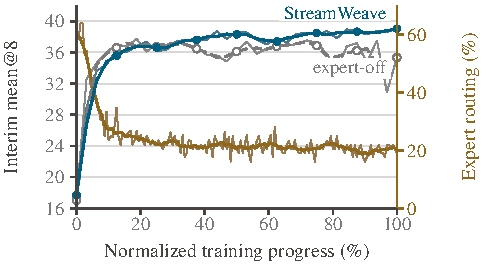
\includegraphics[width=\columnwidth]{figures/figure3.pdf}
  \caption{Learning dynamics and expert-routing rate over normalized training progress; thin curves are observations and thick curves are smoothed trends.}
  \label{fig:learning-dynamics}
\end{figure}

Expert routing falls rapidly as the policy improves early in training and then settles into a persistent tail (Figure~\ref{fig:learning-dynamics}).
The demand for expert supervision narrows but does not vanish: a residual region without reward contrast remains late into training.
Throughout this tail, selected expert inputs enter the one primary update defined in Section~\ref{sec:learning-composition}.

StreamWeave and the expert-off control share the execution stack, policy objective, optimizer, prompt population, and expert access; they differ in whether the expert input selected by an all-failure outcome is consumed.
At an all-failure encounter, the expert-off run receives no group-relative update from that prompt, whereas StreamWeave consumes the selected expert input.
The two runs improve similarly at first and then separate, with the same direction appearing in both average benchmark performance and the held-out all-failure rate.

To separate a local effect on directly routed prompts from a policy-level one, we match prompts by their number of successes at first encounter and compare later encounters.
StreamWeave's improvement from the first encounter to the second exceeds the expert-off control by a weighted mean of $+0.169$ successful rollouts per eight-attempt group.
The difference is positive in all nine strata $k=0,\ldots,8$, is largest in the partial-success region, and remains $+0.159$ at the third encounter.
The pattern is consistent with selective expert contributions supporting both the paired prompt and broader acquisition and retention in the shared policy.
Appendix~C.3 reports the matched population, full stratum-level estimates, standard errors, and later encounters, supporting this interpretation while limiting the evidence to a matched longitudinal comparison.

\paragraph{Choosing the policy-update rule.}
StreamWeave uses Decoupled PPO~\citep{fu2025areal} to correct the policy lag between rollout generation and the start of an update, while PPO Clip-Higher limits how far the policy can move during that update.
Expert inputs are not stale rollouts, but they also update the same policy, so we tested whether this clipping removes useful gradients from policy rollouts.
Holding expert routing, policy-lag correction, and asynchronous execution fixed, we replaced only PPO clipping with a CISPO-style rule that retains gradients outside the PPO clipping range~\citep{minimax2025m1}.
The variant averages 36.8 on the six mathematical reasoning benchmarks, below 38.5 for StreamWeave.
Making the queue fresher reduced early policy lag but did not remove the variant's later training instability.
These results suggest that correcting policy lag does not make PPO clipping redundant; in this setting, clipping remains useful for limiting how far the policy changes during an update.
Appendix~D separates the effects of expert input and the update rule and reports the complete benchmark results together with the queue-freshness and training-history analyses.

\paragraph{Cross-domain reasoning.}
To test whether math-focused expert supervision narrows broader reasoning, we evaluate the same checkpoints on ARC-Challenge, GPQA-Diamond, and MMLU-Pro (Table~\ref{tab:cross-domain}).

\begin{table}[!htbp]
\centering
\begin{tabular}{@{}lrrrr@{}}
\toprule
Model & ARC-C & GPQA-D & \shortstack{MMLU-\\Pro} & Avg. \\
\midrule
\rowcolor{tabbaseline} Base & 5.7 & 3.6 & 3.3 & 4.2 \\
\rowcolor{tabbaseline} Instruct & 54.6 & 27.7 & 30.3 & 37.5 \\
\rowcolor{tabexpert} HPT & \underline{60.5} & 28.8 & \underline{33.9} & \underline{41.1} \\
\rowcolor{tabexpert} SRFT & 48.0 & 24.2 & 28.0 & 33.4 \\
\rowcolor{tabexpert} ReLIFT & 52.8 & 24.5 & 30.2 & 35.8 \\
\rowcolor{tabexpert} LUFFY & 56.5 & 27.0 & \textbf{34.5} & 39.3 \\
\rowcolor{tabasync} Async RL & \textbf{60.8} & \textbf{30.6} & 31.7 & \underline{41.1} \\
\rowcolor{tabours} \textbf{StreamWeave} & 60.2 & \underline{30.3} & 33.2 & \textbf{41.2} \\
\rowcolor{tabexternal} Oat-Zero & 41.9 & 13.5 & 21.5 & 25.6 \\
\rowcolor{tabexternal} ExGRPO & 58.7 & 28.3 & 29.2 & 38.7 \\
\rowcolor{tabexternal} EMPO & 24.8 & 12.3 & 16.2 & 17.8 \\
\bottomrule
\end{tabular}
\caption{Fixed-checkpoint cross-domain reasoning; Avg.\ is the unweighted mean.}
\label{tab:cross-domain}
\end{table}

StreamWeave remains at the same aggregate cross-domain level as Async RL (expert-off) and HPT (sync).
The gain observed over the expert-off control is therefore concentrated in the target mathematical domain, without a clear reduction in cross-domain reasoning.

\subsection{Execution Efficiency with Expert Supervision}
\label{sec:execution-efficiency}

\begin{figure*}[!t]
  \centering
  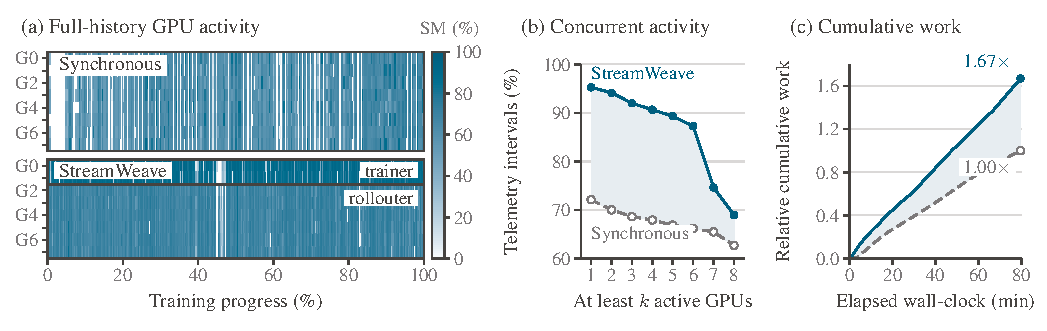
\includegraphics{figures/figure4.pdf}
  \captionsetup{width=\textwidth,singlelinecheck=false}
  \caption{GPU activity and cumulative work under the same 8-GPU budget.
  Panels (a)--(b) normalize each run's non-validation history independently; panel (c) compares the full synchronous run with an equal-length StreamWeave prefix, normalizing work to the synchronous endpoint.}
  \label{fig:execution-efficiency}
\end{figure*}

Because expert supervision remains active late into training (Section~\ref{sec:learning-effectiveness}), the generation workload and completion-tail pressure observed in this regime are persistent execution conditions rather than a transient startup effect.
Two questions follow: whether localizing the wait avoids the execution cost that the complete-group requirement implies, and whether that appears as end-to-end throughput under the same GPU budget.

On the same asynchronous stack, the run with expert supervision exhibits longer responses, wider group tails, and a higher incidence of groups containing rollouts from adjacent policy versions than the expert-off control (Table~\ref{tab:execution}).

\begin{table}[!htbp]
\centering
\begin{tabular}{@{}lrrr@{}}
\toprule
Metric & Ref. & \textbf{Ours} & Change \\
\midrule
\multicolumn{4}{@{}l}{\textit{Generation workload (expert-off reference)}} \\
Response length (tokens) & 896 & \textbf{1,429} & \textbf{$1.59\times$} \\
Longest rollout/group (s) & 6.59 & \textbf{12.79} & \textbf{$1.94\times$} \\
Adjacent-version groups & 2.03\% & \textbf{7.00\%} & \textbf{$3.46\times$} \\
\midrule
\multicolumn{4}{@{}l}{\textit{End-to-end execution (synchronous reference)}} \\
128-group time (s) $\downarrow$ & 46.0 & \textbf{28.0} & \textbf{$-39\%$} \\
Throughput (groups/s) $\uparrow$ & 2.78 & \textbf{4.58} & \textbf{$1.64\times$} \\
\bottomrule
\end{tabular}
\caption{Generation workload and execution efficiency.
 Throughput is pre-routing prompt groups per training-loop second under the same GPU budget, excluding validation and checkpointing.}
\label{tab:execution}
\end{table}

This temporal exposure is not uniform across group outcomes.
Within StreamWeave, 10.0\% of the all-failure groups ultimately assigned to the expert source contain rollouts from adjacent policy versions, the highest rate among the routes.
The region that requires expert supervision therefore interacts most strongly with asynchronous execution not only through its absent reward contrast, but also through when its complete group becomes available.

When all rollouts in a long and uneven group share one execution phase, the slowest trajectory governs pipeline progress.
In the synchronous trace, requests complete in 7.6 seconds on average, but the slowest lasts 23.7 seconds and the generation phase, including post-processing, ends at 25.1 seconds.
Earlier completions cannot launch the next attempt before the phase closes, and model training starts only after generation.
The completion tail therefore constrains both subsequent rollout work and training.

Holding each attempt's execution slot until its group completed is the mildest form of group-level pinning, since it constrains only the eight slots of one group.
Even so, it would have required $1.80\times$ the rollout capacity StreamWeave consumed, and $1.53\times$ on the expert-off control (Table~\ref{tab:pinning}).
StreamWeave does not pay that price.
The two disciplines are also separable in the record: executed occupancy stays flat in the capacity that early finishers return, whereas the occupancy pinning predicts rises steeply with it.
Only one of the two can be a fixed physical pool.

\begin{table}[!htbp]
\centering
\setlength{\tabcolsep}{3pt}
\begin{tabular*}{\columnwidth}{@{\extracolsep{\fill}}lrr@{}}
\toprule
 & \shortstack[r]{If slots\\were pinned} & \shortstack[r]{\textbf{As}\\\textbf{executed}} \\
\midrule
Slot-seconds per group & $8\max_i d_i$ & $\sum_i d_i$ \\
Rollout capacity required & $1.80\times$ & \textbf{$1.00\times$} \\
Occupancy, Q1 $\to$ Q4 & 521 $\to$ 850 & \textbf{363 $\to$ 372} \\
Versions over admission budget & 37 / 190 & \textbf{0 / 190} \\
\bottomrule
\end{tabular*}
\caption{Counterfactual group-level slot-pinning cost from observed attempt durations.
 Occupancy quartiles rank parameter versions by pinned slot-seconds; admission capacity is 768 attempts.}
\label{tab:pinning}
\end{table}

What the requirement does cost is buffer rather than execution.
Attempts held completed inside an unfinished group occupy 7.2\% of the completed-attempt storage budget on time average, against 69.3\% for completed groups awaiting the trainer.
The producer is consequently held off from submitting new work for 23\% of rollout wall-clock, while the trainer's own blocking wait is 2\%.
The pressure therefore follows the trainer's consumption rate rather than group reconstruction.

Figure~\ref{fig:execution-efficiency} shows the hardware-level signature of this design: intervals in which no GPU exceeds the activity threshold fall from 27.9\% to 4.7\%, the mean number of concurrently active GPUs rises from 5.40 to 6.92, and more prompt-group work accumulates over the same wall-clock interval.

StreamWeave reduces the processing time for 128 prompt groups from 46 to 28 seconds and achieves $1.64\times$ prompt-group throughput under the same GPU budget.
Normalized by the response tokens the trainer consumes, the most conservative definition we checked, the gain is $1.30\times$.
Synchronous execution spends 25.1 of its 46.0 seconds generating with all eight GPUs and the remaining 20.9 on computation that cannot begin until generation closes, whereas StreamWeave completes both within 28.0 seconds with six GPUs on its rollouter.
Two connected effects contribute to this gain.
First, model training that follows generation in synchronous execution proceeds concurrently with rollout generation.
Second, immediately refilling a rollout slot after an attempt finishes recovers capacity that would otherwise be lost while early completions wait for the group tail.
Together, these effects recover end-to-end throughput while preserving the complete-group source decision.

Appendix~C.4 documents the group completion tail, including the per-version occupancy comparison behind Table~\ref{tab:pinning}, the synchronous request-level timing, and the route-level version span.
Appendix~C.5 documents the throughput protocol, its token-based recount, and the hardware record.

\FloatBarrier
\section{Conclusion}
\label{sec:conclusion}

StreamWeave confines each dependency created by a complete-group source decision to the interval in which it is needed: group waiting ends when the source is fixed, while the context required to preserve the selected learning role persists only until the corresponding training input is built.

These boundaries retain the selected learning role under one policy objective without making group completion a pipeline-wide synchronization barrier.

Experiments show that the conditions motivating this design persist in practice: generation workload and absent reward contrast concentrate in all-failure groups, expert demand remains late into training, and the observed learning difference extends beyond directly routed prompts.

Under these conditions, StreamWeave achieves reasoning performance comparable to the synchronous quality reference and $1.64\times$ prompt-group throughput under the same GPU budget, while retaining competitive cross-domain reasoning.

Our direct empirical scope is one backbone, one training seed, an 8-GPU budget, and math-centered two-source RLVR with a group-outcome-based source rule.
Within this scope, StreamWeave preserves complete-group source decisions and their selected learning roles while keeping group completion off the pipeline-wide critical path.

\bibliography{references}

\end{document}
